%\qchapter{\textit{You can observe a lot just by watching.} \vskip 0.1em
%  - Yogi Berra}{Related Work}

%"I don't compare 'em, I just catch 'em." - Willie Mays

%Leroy "Satchel" Paige: Quotations: Baseball
%Dont look back. Something might be gaining on you.

%\qchapter{I don't want to play golf.  When I hit a ball, I want someone
%  else to go chase it.  \vskip 0.1em - Rogers Hornsby}{Background and
%  Related Work} 
%\chapter{Related Work}

\qchapter{\textit{Don't look back.  Something might be gaining on you.}  \vskip
0.1em - Leroy ``Satchel'' Paige}{Background and Related Work} 
\label{chap:related}


\cs{I}n~this chapter, we provide an overview of how routing on the
Internet works today, as well as prior work on improving the correctness
and predictability of Internet routing.  We begin in
Section~\ref{sec:structure} with an overview of today's Internet routing
infrastructure: we describe the high-level organization of the Internet
(\ie, as a federation of thousands of independently operated networks
that exchange reachability information) and proceed to describe in
detail the routing protocols that these networks use to achieve global
reachability.
%Finally, in
%Section~\ref{sec:rw_architectures}, we discuss various proposals that
%involve making more fundamental changes or additions to the Internet
%routing architecture.
%
%In Section~\ref{sec:structure}, we describe the structure of the
%Internet and the operation of each independently operated network; we
%also briefly summarize the Internet's competitive landscape.
Section~\ref{sec:bgp} describes how these independently operated
networks exchange routing information with one another using the Border
Gateway Protocol (BGP)~\cite{rfc1771,id-bgp4}, and
Section~\ref{sec:conf} both explains at a high-level how configuration
controls BGP's operation and presents a brief example that describes
Cisco's router configuration language syntax~\cite{www-cisco-ios-master,www-juniper-command-ref}.
Section~\ref{sec:rw_challenges} presents an overview of previous studies
related to the correctness and predictability of Internet routing.
Readers who are already familiar with today's Internet routing protocols and
infrastructure (in particular, BGP) may wish to skip directly to
Section~\ref{sec:rw_challenges}.



\section{Internet Structure and Operation}\label{sec:structure}

Tens of thousands of independently operated networks connect to each
other to form the larger network that we know as ``the Internet''.
These networks are called {\em Autonomous Systems} (ASes), and they
cooperate with one another to provide global connectivity.
Nevertheless, these networks are also in {\em competition} with one
another.  Each one of these ASes contains many routers.  The routers
inside of one of these networks run an internal routing protocol called
an {\em interior gateway protocol} (IGP) that allows them to discover
routes to other destinations within the same AS, including the AS's {\em
border routers}---those routers that connect to neighboring ASes.
Examples of IGPs are Open Shortest Paths First (OSPF)~\cite{rfc1583},
Intermediate System-Intermediate System (IS-IS)~\cite{rfc1142}, and
Routing Information Protocol (RIP)~\cite{rfc1058}.

The Internet is composed of many different types of ASes, from
universities to corporations to regional Internet Service Providers
(ISPs) to nationwide ISPs.  Smaller ASes (\eg, universities,
corporations, etc.) typically purchase Internet connectivity from ISPs.
Smaller regional ISPs, in turn, purchase connectivity from larger
ISPs with ``backbone'' networks.  

The different types of ASes lead to different types of business
relationships, and, hence, different policies for exchanging and
selecting routes.  Although we will expound on these business
relationships later in this chapter, it is reasonable to think of these
business relationships in terms of two types: {\em customer-provider}
and {\em peering}.  Customer-provider relationships involve one AS (the
``customer'') paying another (the ``provider'') in exchange for carrying
its traffic to some portion of the Internet's destinations (often, every
destination outside of its own network)~\cite{Gao2001}.  In today's
Internet routing, 
{\em a route advertisement is an implicit agreement for carrying
traffic}.  The process of carrying traffic between two different ASes is
called ``providing transit''.  In these relationships, the customer pays
the provider for transit, regardless of the direction in which the
traffic is flowing.

In {\em peering} relationships, two ASes agree to trade traffic to
various destinations at no cost.  Typically, a pair of ASes will
recognize that it is more cost-effective to directly exchange traffic to
(some or all of) one another's customers, rather paying to send the
traffic through one or more provider ASes.  For those interested in a
more detailed treatment of the business aspects of peering, Norton
provides an excellent overview of peering and the decision parameters
that ASes must consider for deciding whether to peer~\cite{Norton2000}.


%%%%%%%%%%%%%%%%%%%%%%%%%%%%%%%%%%%%%%%%%%%%%%%%%%%%%%%%%%%%

\section{Internet Routing: The Border Gateway Protocol}\label{sec:bgp}

In this section, we describe the operation of the Border Gateway
Protocol, version 4 (BGP)~\cite{rfc1771,id-bgp4}.  The first two
sections describe the basic 
operation of the protocol---the protocol state machine, the format of
routing messages, and the propagation of routing updates---all of which
is defined in the protocol standard~\cite{rfc1771}.  A noteworthy aspect
of BGP is that many of the features that determine the behavior of the
global routing system are {\em not} standardized.  Later in this section, we
discuss two important non-standard aspects of Internet routing:
the route selection process and configuration languages.

To ensure reliable delivery of routing messages, all BGP sessions
exchange information using the Transmission Control Protocol
(TCP)~\cite{rfc793} 
(the same transport protocol used by common Internet applications that
require reliable message delivery, such as email and the Web).  Like
TCP, BGP also has a protocol state machine. Because BGP's state machine
is primarily concerned with enabling two routers to establish a
communication channel with one another and is unconcerned with the
routing messages themselves (all routing messages are exchanged in the
``{\tt ESTABLISHED}'' state), we forgo further description of BGP's
state machine.  For a detailed description of BGP's finite state machine
(including how timers can affect the transition between protocol states,
and when these timers are reset), see the protocol standard and related
documents~\cite{Beijnum2002, rfc1771, Stewart98}.


%% \begin{figure}
%% \centering\epsfig{file=figures/bgp_fsm.eps, width=0.3\linewidth}
%% \caption[BGP's finite state machine]{BGP's finite state machine.
%% Routing updates are exchanged 
%% between two routers that are in the {\tt ESTABLISHED} state.}
%% \label{fig:bgp_fsm}
%% \end{figure}

%% Figure~\ref{fig:bgp_fsm} provides an overview of BGP's finite state
%% machine and the messages exchanged between two routers to establish a
%% BGP session.  


%% Each router that runs BGP initially begins in the idle
%% state, and listens for connections on port 179.  A neighboring router may
%% then try to initiate a TCP connection to that router; when that router
%% attempts to establish a connection, it transitions to the {\tt CONNECT}
%% state.  If the connection succeeds, the router sends an {\tt OPEN}
%% message to its neighbor and transitions to the {\tt OPEN\_SENT} state
%% and waits to receive an {\tt OPEN} message from its neighbor.  If the
%% connection fails, the router returns to the {\tt ACTIVE} state,
%% whereupon it will listen for connections on port 179, wait for a retry
%% timer to expire and re-attempt to establish a TCP connection
%% (transitioning again to the {\tt CONNECT} state).  
%% %
%% Upon receiving an {\tt OPEN} message from its neighbor in the {\tt
%% OPEN\_SENT} state, the router checks the message for correctness.  If
%% the message is not correct, the router will send a {\tt NOTIFICATION}
%% message, close the connection, and return to the {\tt IDLE} state.  If
%% the message has no errors, the router sends a {\tt KEEPALIVE} message
%% back to the router that sent the {\tt OPEN} and changes its state to
%% {\tt OPEN\_CONFIRM}, where it waits for either a {\tt KEEPALIVE} or {\tt
%% NOTIFICATION} from the neighboring router.  If the router receives a
%% {\tt KEEPALIVE}, it then transitions to the {\tt ESTABLISHED} state;
%% otherwise, it returns to the {\tt IDLE} state.

%% The {\tt ESTABLISHED} state is the state of the protocol that the
%% routers are in when BGP is in its normal mode of operation---that is,
%% when it is exchanging routing {\tt UPDATE} messages (which we will
%% henceforth simply call {\em updates}).  The next section describes these
%% routing updates in more detail.  In the {\tt ESTABLISHED} state, routers
%% also exchange {\tt KEEPALIVE} messages to indicate that the link between
%% the two routers is still operational (since TCP provides no such monitoring
%% capability).


\subsection{Route Propagation: Announcements and
Withdrawals}\label{sec:propagation} 

\begin{table}
\begin{tabular}{l|p{3.45in}}
{\bf Route Attribute} & {\bf Description} \\ \hline
{\em Next Hop} & 
\parbox{3.45in}{
\vspace*{0.05in}
IP Address of the next-hop router along
the path to the destination. \\ On eBGP sessions, the next hop is set to
the IP address of the border router. On iBGP sessions, the next hop
is not modified.
\vspace*{0.05in}
} 
\\ \hline
{\em Multiple-Exit Discriminator (MED)} & 
\parbox{3.45in}{
\vspace*{0.05in}
Used for comparing two or more
routes from the same neighboring AS.  That neighboring AS can set the
MED values to indicate which router it prefers to receive traffic for
that destination. \\ {\em By default, not comparable among routes from
different ASes.}
\vspace*{0.05in}
} 
\\ \hline
{\em Local Preference} & 
\parbox{3.45in}{
\vspace*{0.05in}
This attribute is the first criteria used to
select routes.  It is not attached on routes learned via eBGP sessions,
but typically assigned by the import policy of these sessions;
preserved on iBGP sessions.}
\vspace*{0.03in}
\\ \hline
\end{tabular}
\caption{Commonly used BGP route attributes.}
\label{tab:route_attributes}
\end{table}

To understand how routers exchange routes using BGP, it is important to
keep in mind several defining features.  First, BGP is a {\em
path vector} protocol.  In a path vector protocol, routing updates
contain the sequence of ASes that the routing advertisement traversed
(\ie, the {\em AS path}).  BGP includes AS path information to avoid the
``counting to infinity'' problem that exists in traditional distance
vector protocols~\cite{Halabi2001}.  The AS path allows an AS that
learns a route to determine whether or not it has already heard the
route by checking to see whether its own AS is contained in the
path.\footnote{Contrary to what many believe, the AS path is {\em not}
intended to indicate the sequence of ASes that traffic will traverse en
route to the destination, although the AS path and this sequence of ASes
often match~\cite{Mao2003}.}  Destinations are represented
as IP {\em 
prefixes}, as described in Section~\ref{sec:intro:overview}.  A BGP
route announcement has several associated route attributes in addition
to the AS path, many of which are obsolete.  The most relevant BGP route
attributes are summarized in Table~\ref{tab:route_attributes}.


Second, BGP maintains state about the routing topology: routers do not
periodically ``refresh'' routing reachability information; rather,
routing messages reflect only {\em changes} in this information.  These
changes in information are reported with two types of routing updates:
{\em announcements} and {\em withdrawals}.  To announce that it can
reach a destination (or to change the existing route to a destination),
a BGP-speaking router sends an announcement for that destination to a
neighboring router.  If a destination is no longer reachable, a router
sends a withdrawal message to the neighboring router.  That neighboring
router may be located either in a neighboring AS or in the same AS.  BGP
sessions between routers in the same AS are called {\em internal BGP
(iBGP)} sessions, and those between routers in different ASes are called
{\em external BGP (eBGP)} sessions.  The goal of eBGP is to allow ASes
to exchange reachability to destinations in each other's networks; the
goal of iBGP is to ensure that {\em every} router within an AS learns at
least one route to every destination.


\subsection{Route Selection (And How Operators Can Control
It)}\label{sec:bg:route_selection} 

\begin{table}
\begin{small}
\begin{center}
\begin{tabular}{r|l|l} 
{\bf Step} & {\bf Criterion} & {\bf How Configuration Can Manipulate
This Step} \\ \hline
1 & Highest local preference & AS's import policy \\
2 & Lowest AS path length & Neighboring AS can ``prepend'' additional hops \\
{\color{Gray} 3} & {\color{Gray} Lowest origin type}   & {\color{Gray} Obsolete} \\
4 & Lowest MED (with {\em same\/} next-hop AS) & Neighboring AS's export
policy \\
5 & eBGP-learned over iBGP-learned  & ---\\
6 & Lowest IGP path cost to egress router & AS's IGP topology \\
7 & Lowest router ID of BGP speaker & --- \\
\end{tabular}
\end{center}
\end{small}
\caption{Steps in the BGP route selection process.}
\label{tab:background:decision}
\end{table}


Any given router may learn multiple routes to a destination (\ie, IP
prefix), but must ultimately select a single best route along which to
forward traffic to that destination.  The route selection process
determines which route each router selects.  The original standards
document does not specify the route selection process~\cite{rfc1771},
but the route selection process has since become a {\em de
facto} standard~\cite{www-cisco-bgp-path, id-bgp4}.

Table~\ref{tab:background:decision} summarizes the route selection
process, as well 
as how network operators can use routing configuration to try to
influence which route each router selects at each step of the process.
First, given multiple routes to the same destination (\ie, IP prefix), a
router will select the route with the highest ``local preference''
value.  As this attribute is not set by the receiving AS's import policy
and is the first step in the decision process, it provides the operator
direct influence over which route the router ultimately selects
to this destination.  Operators typically use the local
preference attribute to implement the types of policies described in
Table~\ref{tab:business}.  

\begin{figure}
\centering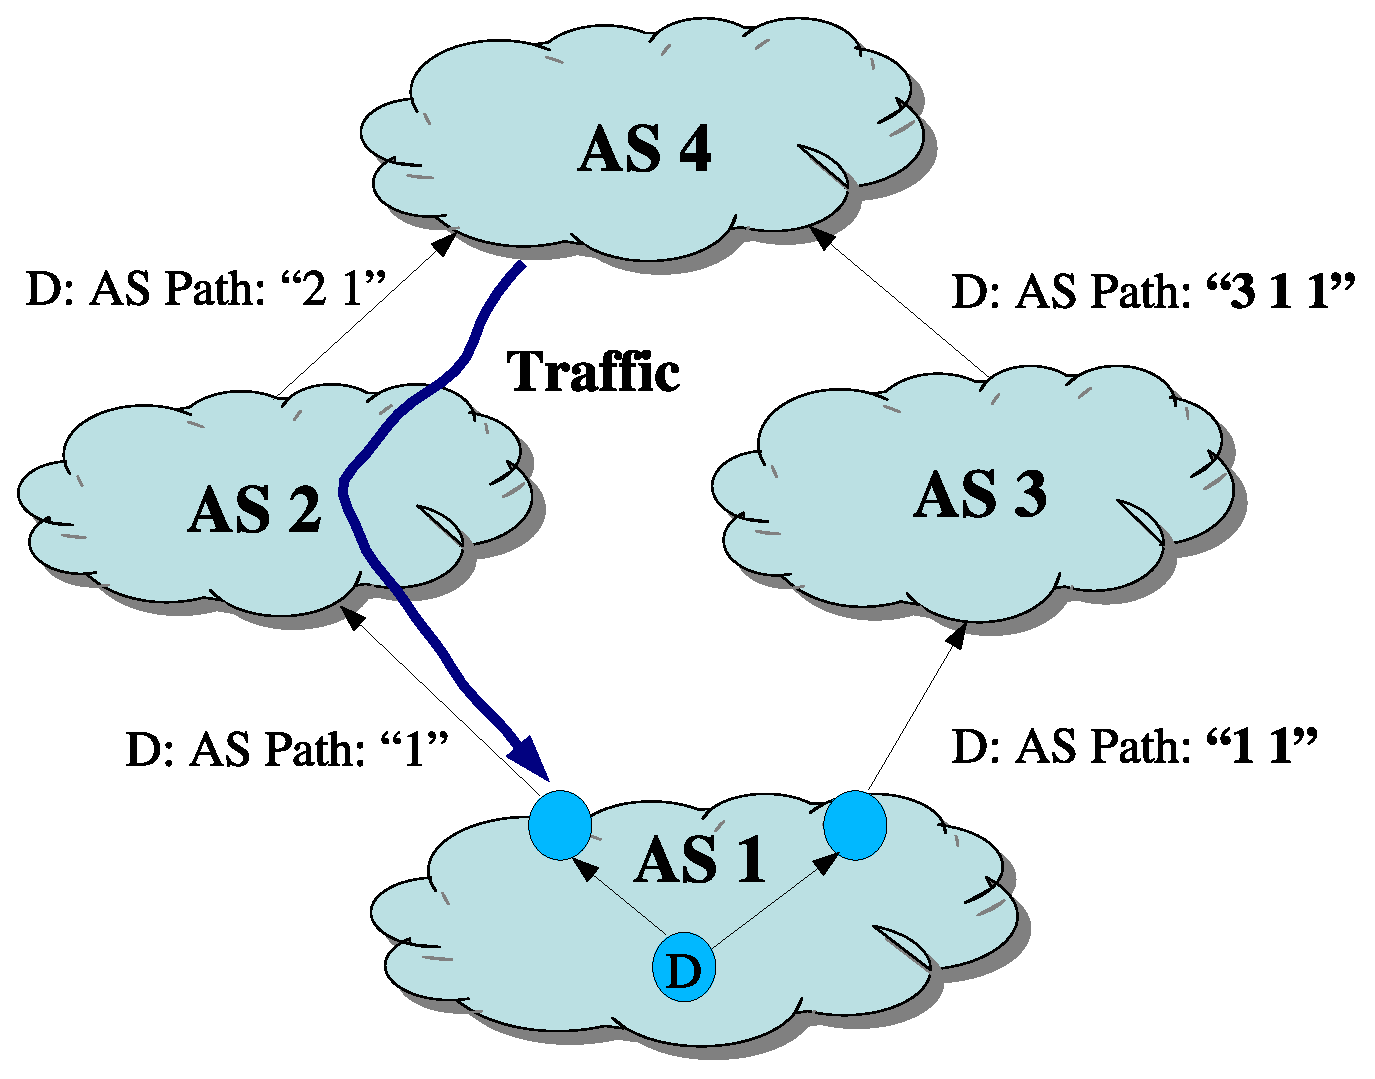
\epsfig{file=figures/prepend.eps, width=0.65\linewidth}
\caption[The use of AS path prepending to control inbound
traffic]{Operators sometimes use {\em AS path prepending} to try to 
control inbound traffic.}
\label{fig:prepend}
\end{figure}


Among multiple routes to a destination with equal local preference
values, a router will 
select the route with the shortest AS path length, which is simply
the number of AS-level hops in the AS path.  This criterion is 
a crude approximation for selecting a shortest path to the destination.
In practice, a
path with the fewest number of ASes does not correspond to the
path with the lowest latency, or to the path with the fewest number of
IP-level hops.  However, network operators do use routing configuration
to try to influence route selection using a technique called {\em AS
path prepending}, which artificially increases the length of a route's AS
path by adding the same AS number to the path multiple times.
Figure~\ref{fig:prepend} illustrates this practice: AS~1 wants inbound
traffic for $D$ to arrive via AS~2, rather than via AS~3.  To express
this preference, it
prepends an additional ``$1$'' to the AS path for its route to $D$ when
it advertises the route to AS~3.  If an upstream AS, say AS~4, learns
two routes to $D$---\ie, one via AS~2 and the other via AS~3---it will
prefer the route with the route via AS~2 because it has a shorter AS path
length (assuming it does not assign a higher local preference to routes
learned from AS~3).  Of course, this technique for controlling inbound
traffic has limited utility in practice, because AS~1 does not control
the policies (\ie, local preference values) of other ASes, and it also
cannot easily determine the AS path lengths that an upstream might see
for its route advertisements~\cite{Gao2005}.  Despite the fact that
prepending is widely used, the technique is largely ad hoc and of
only limited utility~\cite{Feamster2003e, Quoitin2005}.


If a router has two routes to the same destination with equal local
preference and AS path length, the router will then select the route with the
lowest ``origin type''.  Because this route attribute is deprecated, in
practice, 
route selection then typically falls to selecting the route with the
lowest multiple exit discriminator (MED) value.  If a neighboring AS
advertises a route to an AS at multiple locations, it may attach
different MED values to these routes to indicate that it prefers a
neighboring AS to use one exit point over another.  For example, in
Figure~\ref{fig:rw_med}, AS~1 is indicating to AS~2 that it wishes to
have traffic sent to destination $d$ via the exit point in New York
over the one in San Francisco by advertising the route to $d$ with a larger
MED value over the BGP session in San Francisco.  By default, the MED value is
only comparable among routes learned from the same neighboring AS, since
different ASes may use different ranges of MED values to specify
preferences over routes.  As we will see later in this dissertation, the
fact that the MED attribute is not comparable across all routes creates
many problems for correctness and predictability.

\begin{figure}
\begin{minipage}{0.48\linewidth}
\centering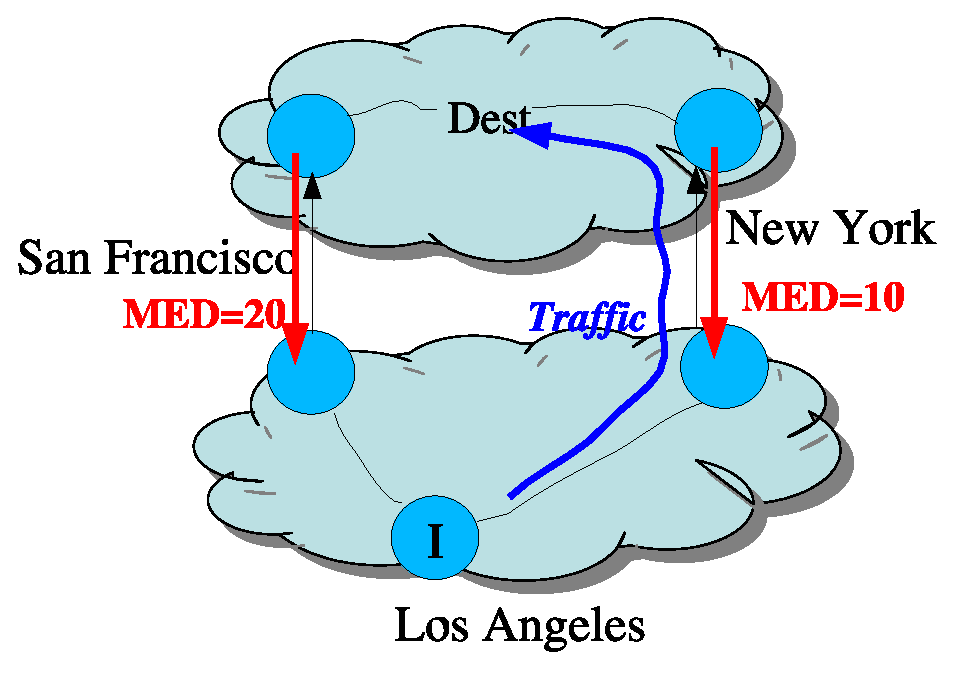
\epsfig{file=figures/med.eps, width=\linewidth}
\caption[The use of the MED attribute to control inbound traffic]{A
neighboring AS can advertise routes to a destination with 
different MED values at different locations to control the exit point
that routers in a neighboring AS uses to send traffic for that
destination.  When $I$ learns both routes, it will select the route
learned via the router in New York (and, thus, it will send traffic that
way).}
\label{fig:rw_med}
\end{minipage}
\hfill
\begin{minipage}{0.48\linewidth}
\centering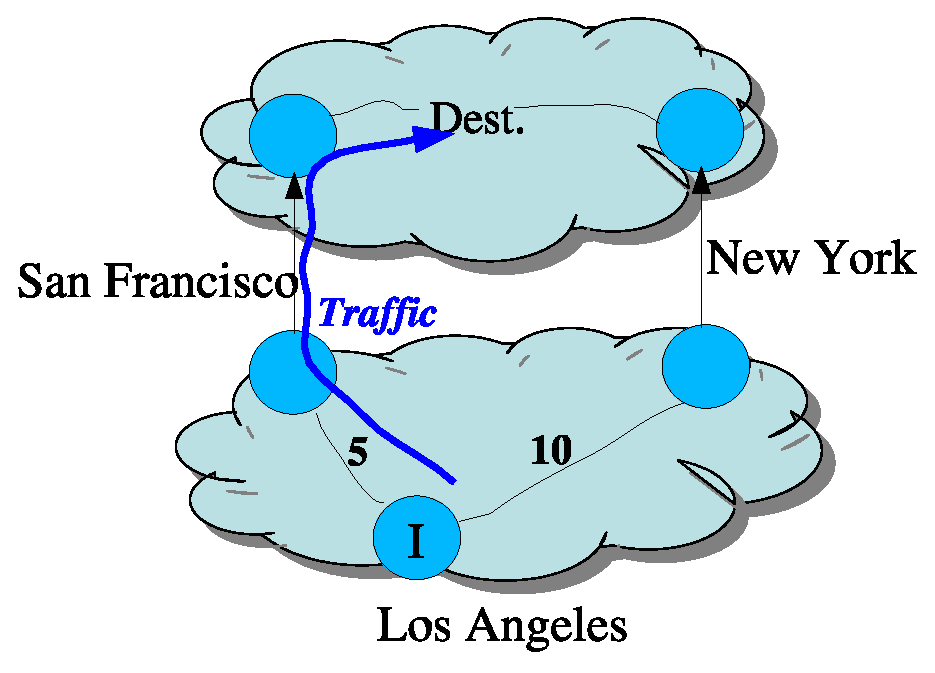
\epsfig{file=figures/hotpotato.eps, width=\linewidth}
\caption[How the IGP implements ``hot potato'' routing]{If router $I$ learns two or more routes that are equally good
up through Step~5 in Table~\ref{tab:background:decision}, it will select the route
whose next hop has a shortest IGP path cost.  IGP path costs are shown as
numbered edges; these path costs often correspond to geographic distance.}
\label{fig:background:hotpotato}
\end{minipage}
\end{figure}

%\begin{figure}
%\end{figure}


If multiple routes remain after Step~4, a router will prefer a route
that it learned via eBGP over one that it learned via iBGP.  If multiple
routes still remain, the router will prefer the route whose next-hop IP
address is ``closest'' in the internal routing topology (\ie, the
shortest IGP path).  This step allows a network to achieve what is
commonly referred to today as ``hot potato routing'': the process by
which an AS tries to offload traffic to neighboring ASes as quickly as
possible.\footnote{``Hot potato routing'' was initially coined by Paul
Baran for {\em all} routing techniques where nodes would forward
messages as quickly as possible~\cite{hafner1996}.  This notion stood in
contrast to quintessential ``store and forward'' networks like the
telegraph.  In these systems, the electrical signal would dissipate
after some distance.  As such, relay nodes would transcribe the message
in Morse code, and an operator would then re-feed the ticker to
the relay node, which would regenerate the electrical signal.}  
Figure~\ref{fig:background:hotpotato} illustrates this mechanism.  A network
operator could conceivably control interdomain traffic by adjusting edge
weights in the IGP. Unfortunately, updates in the IGP topology
can cause unexpected and unwanted shifts in BGP routes, potentially
affecting large volumes of traffic~\cite{teixeira2004b}.

If multiple routes remain after the IGP tiebreak, the routers may break
ties in a number of ways.  This final tiebreak is usually based on the
``router ID'' of the router that advertised the route, although other
tiebreaking mechanisms are sometimes used, such as selecting the ``most
stable'' route (\ie, the one that has been advertised for the longest
period of time).

A key problem operators face is determining which route each router in
the AS will select.  It might seem that this process might be as simple
as taking the set of eBGP-learned routes for a destination and applying
the process in Table~\ref{tab:background:decision} at each router.  In
fact, predicting the outcome of this process is not so simple:
Chapter~\ref{chap:sandbox} is 
dedicated to solving this problem.


\subsection{Putting It Together: How Traffic Gets from Here to There}

We now describe how IGP, iBGP, and eBGP act in
concert to establish routes between various endpoints.  One can think of
a route in terms of two distinct phases: (1)~the route to some exit (or
``egress'') router in that AS (or to the ultimate destination, if the
destination is located in the same AS) and (2)~the route from the egress
point to the appropriate next-hop AS.

%\subsubsection{Routing Within a Single AS: Internal BGP (iBGP) and IGP}

An example of the route to a destination in a router's routing table is
shown in Figure~\ref{fig:bgpex}: each destination prefix has a next-hop
IP address to which to send traffic.  If the destination is in a different
AS and the router is not an egress router, then that next hop is
typically the IP address of an egress router.  The BGP route selection
process determines which egress router each router sends
traffic to: each router in the AS may learn a route for some destination
from one or more egress routers, but ultimately selects only one of
those routes.  The AS's IGP is then responsible for determining the
route from that router to the egress router named by that next-hop IP
address.

If, on the other hand, the destination is in a remote AS and the router
is an egress router, the router will either select a route with a next
hop that is in a neighboring AS, or it will select a route learned from
a different egress router and rely on the AS's IGP to forward traffic to
the egress router with that next-hop IP address.


%%%%%%%%%%%%%%%%%%%%%%%%%%%%%%%%%%%%%%%%%%%%%%%%%%%%%%%%%%%%

\section{Internet Routing Configuration}\label{sec:conf}

Internet routing's true complexity
lies in the fact that so many aspects of the routing protocol's
operation are manipulable with configuration.  
As discussed in Chapter~\ref{chap:intro}
(Section~\ref{sec:intro:config}), and as we will see throughout this
dissertation, many of the problems faced by the Internet routing system result
from the protocol's configurability.


This section provides background on Internet routing configuration.
Internet routing configuration languages typically have thousands of
distinct commands~\cite{www-cisco-ios-master}; the reader will be
pleased to learn that we will not survey all of them here.  Rather, we
first classify the {\em semantics} of routing configuration into three
main operations: ranking, filtering, and dissemination.  We then provide
a brief example of Cisco router configuration {\em syntax} to
demonstrate how a network operator can implement these
operations in practice.

\subsection{Semantics: Ranking, Filtering, Dissemination}
\label{sec:semantics}

\begin{figure}
%\centering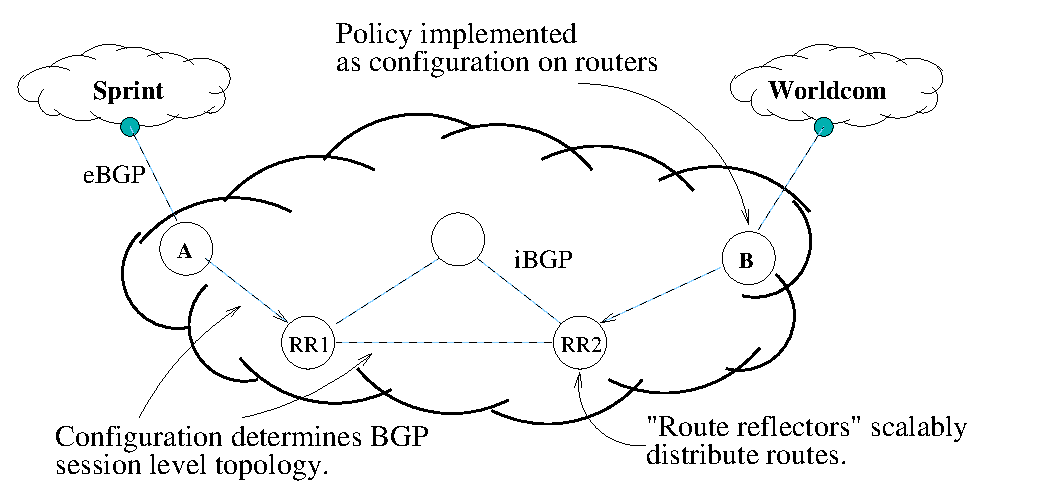
\epsfig{file=rcc/figures/overview.eps, width=\linewidth}
\centering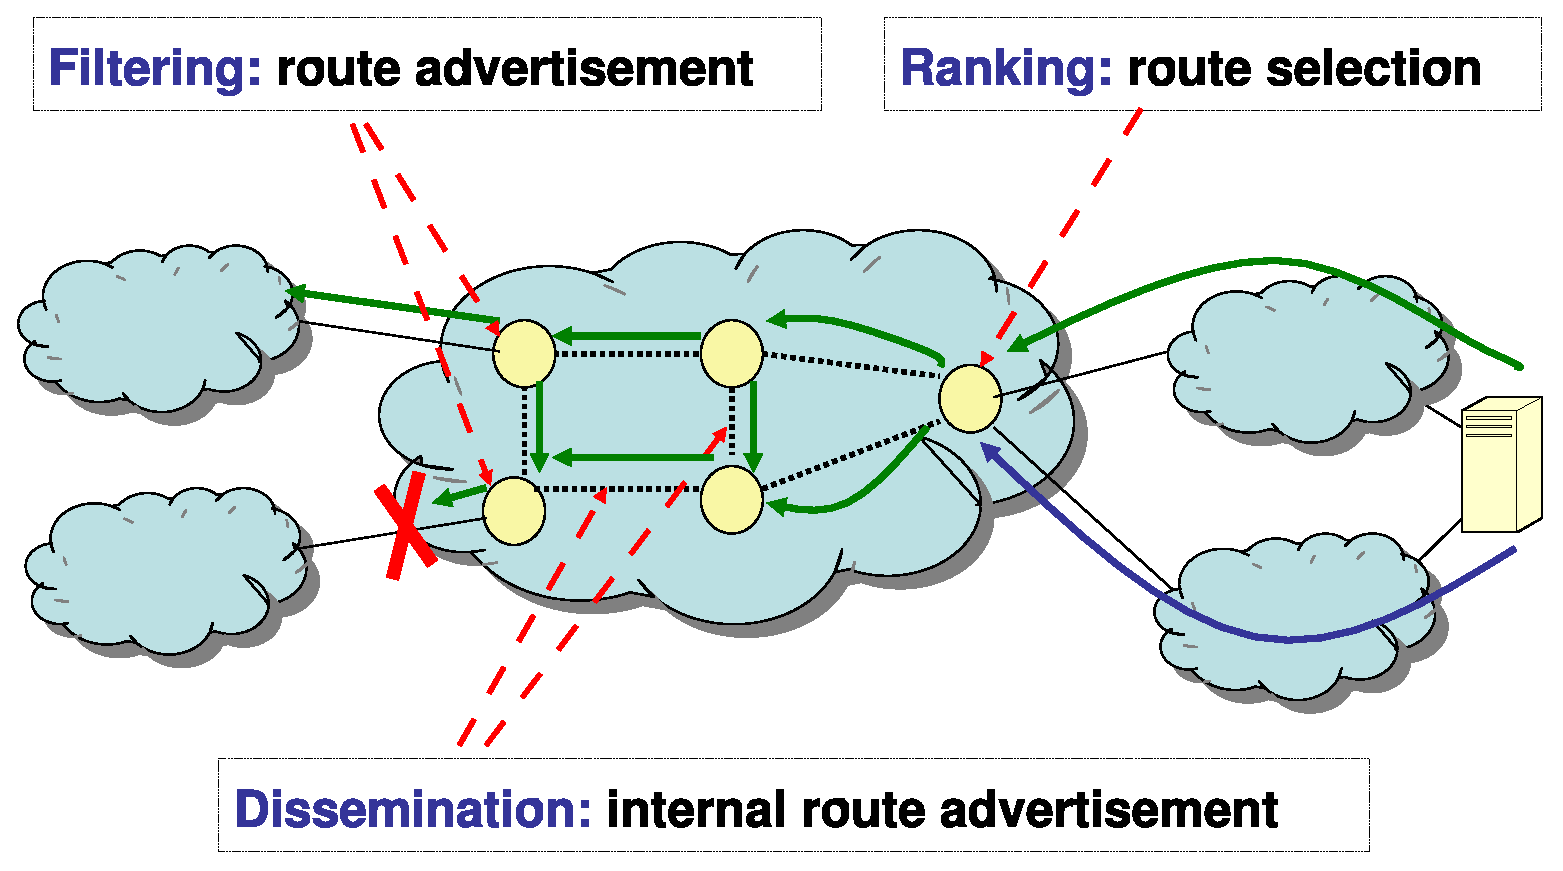
\epsfig{file=rcc/figures/factoring2.eps, width=\linewidth}
\caption{BGP configuration semantics.}
\label{fig:overview}
\end{figure}

Internet routing configuration allows the routing protocol to achieve
two important goals:
\begin{enumerate}
\itemsep=-1pt
\item {\em Policy.}  
Internet routing must be flexible enough to implement complex business
relationships.  Internet routing configuration provides network
operators the ability to encode these policies in router configurations.
\item {\em Scalability.} The Internet must scale to a large number of
hosts, routers, and ASes.  To achieve this scalability, Internet
routing configuration allows an operator to specify various ways for the
routing protocol to aggressively aggregate routing information (\eg,
using route reflection).
\end{enumerate}

The rest of this section describes how routing configuration's three
main operations---ranking, filtering, and dissemination---facilitate
the expression of complex business policies and provide options for
achieving scalability.  We also briefly explain how each of these
operations can affect the correctness and predictability of Internet
routing. 

\subsubsection{Policy: Ranking and Filtering}

The bilateral business relationships established between ASes (as
described in Section~\ref{sec:structure}) imply that the {\em policy}
afforded by Internet routing configuration should provide a network operator
two degrees of control: (1)~which route each router in the AS should
prefer, given multiple routes to a destination ({\em ranking});
(2)~which routes should be advertised to which neighboring ASes ({\em
filtering}).  Table~\ref{tab:business} summarizes these common practices
for both ranking and filtering.  Although these practices constitute the
conventional wisdom for how ASes operate, Section~\ref{sec:bg_stability}
presents examples of some common deviations from these practices.  We
now explain these practices in more detail in this section.

\begin{table}
\centering\begin{tabular}{p{1in}||p{2.35in}|p{2.05in}}
\parbox{1in}{{\em Type of \\neighboring AS}}  & {\bf Ranking} & {\bf
Filtering} \\ \hline  
{\bf Customer} & Most preferred & 
Advertise to all other ASes \\ 
{\bf Peer} & Less preferred than routes through customer, more preferred
than routes through provider & Advertise to customer ASes \\
{\bf Provider} & Least preferred & Advertise to customer ASes
\\
\end{tabular}
\caption[Common business relationships and practices between
ASes]{Common business relationships and practices between ASes on the 
Internet today.  Although this table summarizes the conventional wisdom
of how ASes commonly interact today, Section~\ref{sec:bg_stability}
describes several violations of these practices.}
\label{tab:business}
\end{table}

Because a customer pays a provider per unit traffic regardless of the
direction the traffic is flowing, it is to an AS's advantage to select
routes to destinations via its customer ASes, given the option.
Similarly, an AS would typically prefer to send traffic through one of
its peers (which it can do at no additional cost) versus sending traffic
via one of its providers (which will charge it for the service of
carrying that traffic).


A router's configuration can prevent a certain route from being accepted
on inbound or readvertised on outbound.  Configuring filtering is
complicated because global behavior depends on the configuration of
individual routers. An AS will
typically advertise its entire set of routes to its customers (who it
will gladly charge to carry traffic to any of those destinations) but
will only advertise to one of its peers the routes that it learned from
one of its customers.  On the other hand, an AS will not advertise
routes that it learns from one if its providers to another one of its
providers: doing so would cause that AS to provide transit between two
of its providers and pay {\em both} of its providers to boot!


\subsubsection{Scalability: Dissemination}\label{sec:dissemination}


\begin{figure}
\centering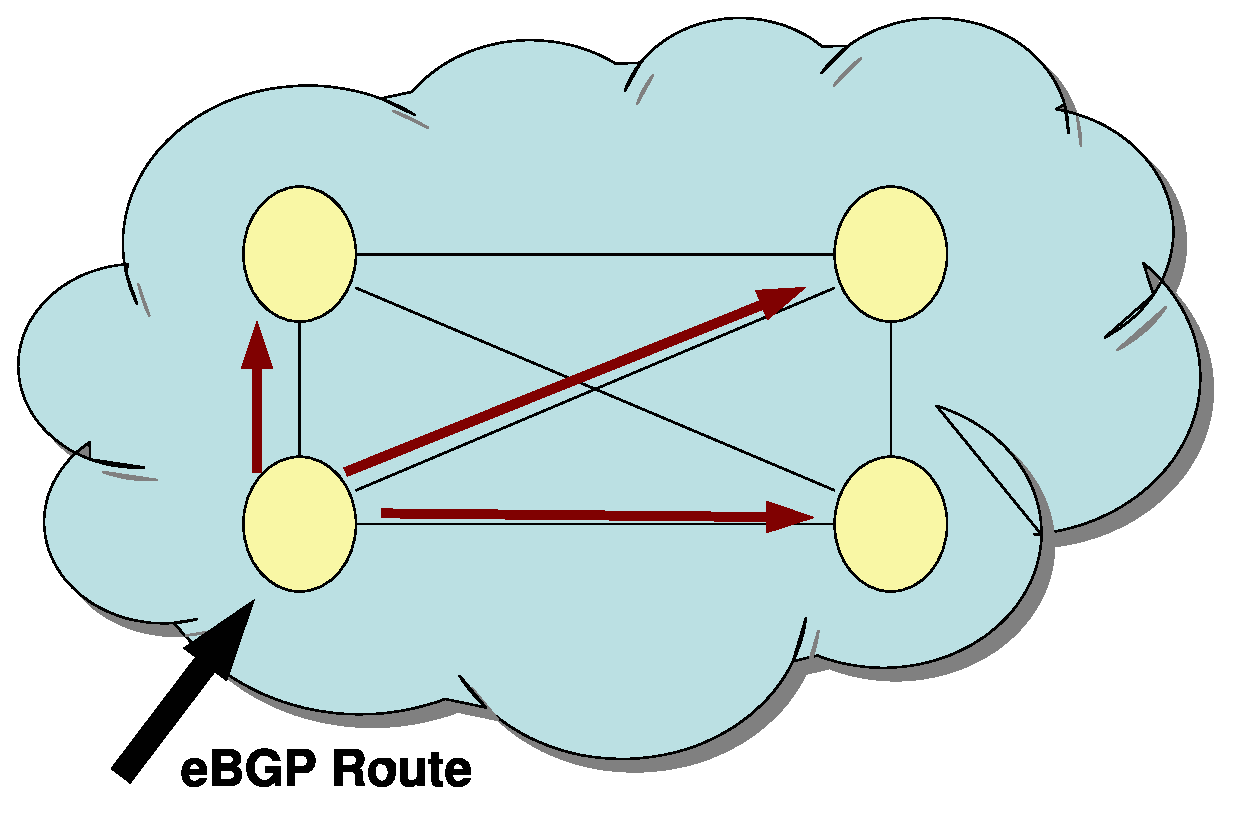
\epsfig{file=figures/fullmesh.eps, width=0.4\linewidth}
\caption[Internal BGP configuration for small ASes: ``full mesh''
topology]{Small ASes establish 
a clique (or ``full mesh'') of iBGP 
sessions.  Each circle represents a router within an AS.  Only
eBGP-learned routes are readvertised over iBGP sessions.}
\label{fig:fullmesh}
\end{figure}

\begin{figure}
\centering
\subfigure[Routes learned from clients are readvertised over all iBGP
sessions.]{
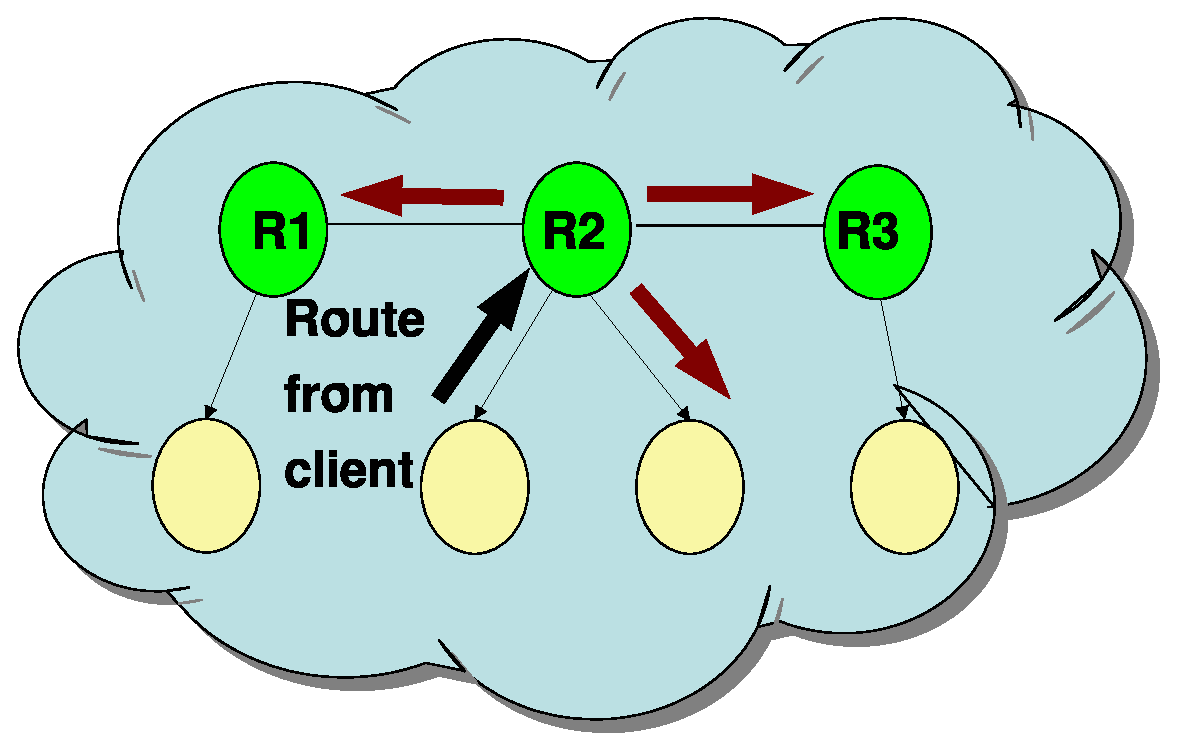
\epsfig{file=figures/rr1.eps, width=0.45\linewidth}}\hfill
\subfigure[Routes learned from non-clients are readvertised to clients only.]{ 
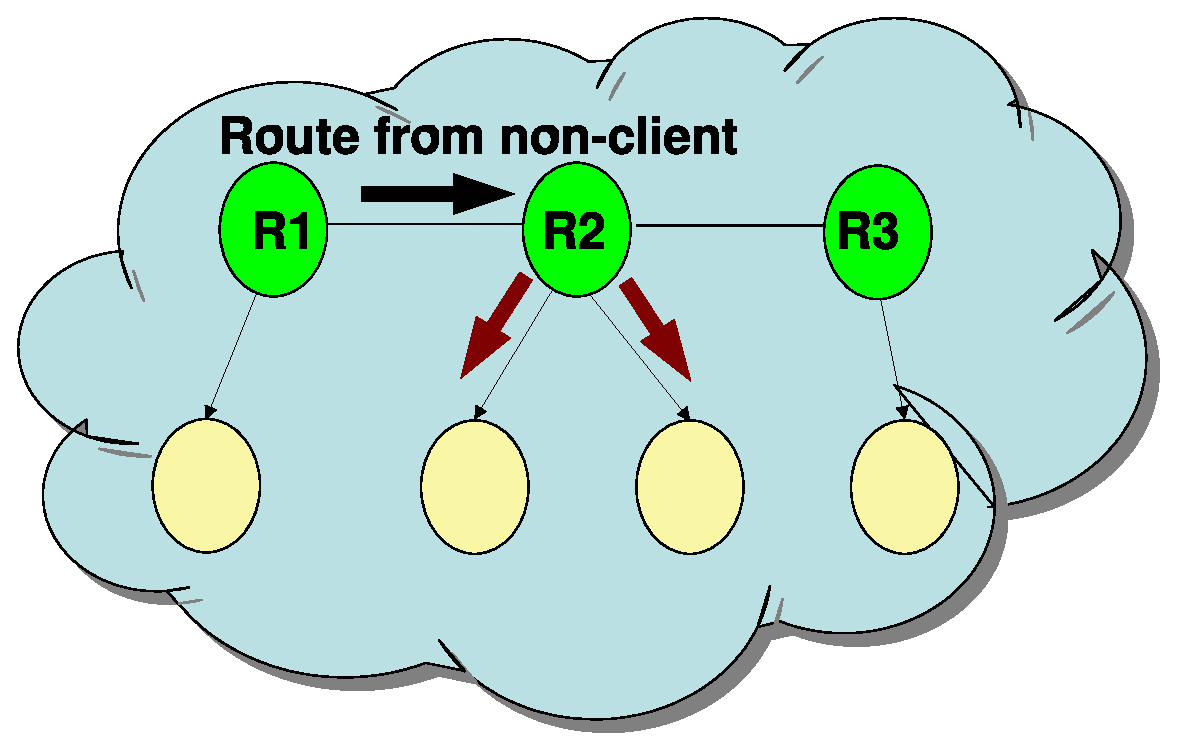
\epsfig{file=figures/rr2.eps, width=0.45\linewidth}}
\caption[Internal BGP configuration for large ASes: route reflector
topology]{Larger ASes commonly use route reflectors, which advertise
some iBGP-learned routes as described above. Directed edges between routers
represent iBGP sessions from route reflectors to clients (\eg, router
$R2$ is a route reflector with two clients). As in
Figure~\ref{fig:fullmesh}, all routers readvertise eBGP-learned routes
over all iBGP sessions.}
\label{fig:ibgp_rr}
\end{figure}

A router's configuration controls the {\em dissemination} of routes
within the AS and between neighboring ASes by allowing each router to 
establish BGP sessions with neighboring routers.  Router configuration
allows an the router to establish two types of BGP sessions: those to
routers in its own AS (iBGP) and those to routers
in other ASes (eBGP).  A small AS with only two or
three routers may have only 10 or 20 BGP sessions, but large backbone
networks may have more than 10,000 BGP sessions, more than half of
which are iBGP sessions.  

BGP messages propagate differently depending on whether the update
is propagating over an eBGP session or an iBGP session.  An eBGP session
is typically a {\em point-to-point} session: that is, the IP addresses
of the routers on either end of the session are directly connected with
one another and are typically on the same local area network.  There
are, of course, exceptions to this practice (\ie, ``multi-hop
eBGP''~\cite{www-ebgp-multihop}), but directly connected eBGP sessions
is normal operating procedure.  In the case where an eBGP session is
point-to-point, the next-hop attribute for the BGP route is guaranteed
to be reachable, as is the other end of the point-to-point connection.
A router will advertise a route over an eBGP session regardless of
whether that route was originally learned via eBGP or iBGP.

On the other hand, an iBGP session may exist between two routers that
are {\em not} directly connected, and it may be the case that the
next-hop IP address for a route learned via iBGP is more than one
IP-level hop away.  In fact, as the next-hop IP address of the route is
typically one of the border routers for the AS, this next hop may not
even correspond to the router on the other end of the iBGP session, but
may be several {\em iBGP} hops away.  In iBGP, the routers thus rely on
the AS's internal routing protocol (\ie, its IGP) to both (1)~establish
connectivity between the two endpoints of the BGP session and
(2)~establish the route to the next-hop IP address named in the route
attribute.  

The session-level iBGP topology determines how BGP routes propagate
through the network.  By default, a router will only readvertise a route
on an iBGP session if it learned that route via an eBGP session.  This
constraint requires that every router in an AS have an iBGP session with
every router that learns routes via eBGP (typically every other router),
as shown in Figure~\ref{fig:fullmesh}; \ie, those routers must form a
clique (the networking community commonly refers to this configuration
as a ``full mesh'' iBGP topology).

ASes with a small number of routers are often configured in a full mesh
iBGP topology, but a fully meshed iBGP topology requires $O(n^2)$
sessions for an AS with $n$ eBGP-speaking routers, which does not scale
well.  Two alternatives have been proposed to solve these problems:
route reflection~\cite{rfc2796} and confederations~\cite{rfc3065}.  To
improve scalability, larger networks typically use {\em route
reflectors}.  A route reflector selects a single best route and
announces that route to all of its ``clients''.  A route reflector is
defined by the fact that it has {\em client} routers, and it
readvertises its iBGP-learned routes to some other routers in the same
AS according to the following rules: (1)~if a route reflector learns a
route via eBGP or via iBGP from one of its clients, it readvertises that
route over all of its sessions to its clients; (2)~if it learns the
route via iBGP from a router that is not one of its clients, it
readvertises the route to its client routers {\em but not over any other
iBGP sessions}.  Figure~\ref{fig:ibgp_rr} shows an example route
reflector hierarchy and how routes propagate from various iBGP sessions.

Configuring an iBGP topology correctly is relatively difficult; we
discuss iBGP misconfiguration in more detail in
Section~\ref{sec:visibility}.  Incorrect iBGP topology configuration can
create many types of incorrect behavior, including persistent forwarding
loops and oscillations~\cite{Griffin2002}.
%Route reflection creates problems both for correctness and for modeling.
Route reflection causes problems with correctness because not all route
reflector topologies are guaranteed to propagate a route learned via an
eBGP session (\ie, not all iBGP topologies satisfy path visibility).  We
describe this problem in more detail in Chapter~\ref{chap:rcc}.  

Route reflectors also complicate predictability because they prevent each
router from learning every BGP route.  Thus, the BGP route that each
router ultimately selects may not be the same route that it would have
selected had it learned every BGP route for that destination (as it
would have in a full mesh iBGP topology).  This property makes route
prediction 
more difficult because the routes that some routers ultimately select
depend on the routes that other routers in the AS select.  Efficiently
computing the route that each router selects thus requires determining
these dependencies and ``visiting'' the routers within the AS in the
correct order.  Chapter~\ref{chap:sandbox} describes in more detail how
route reflection complicates predicting route selection within an AS.

Dissemination primarily concerns flexibility in iBGP configuration, but
the configuration may also {\em manipulate} route attributes when
disseminating routes for one of the following reasons: (1)~controlling
how a router ranks candidate routes, (2)~controlling the ``next hop'' IP
address for the advertised route, and (3)~``tagging'' a route to control
how the ranking and filtering functions on other routers treat it.


\subsection{Syntax: Routing Configuration Languages}\label{sec:configuration}

\begin{figure}
{\tt
        router bgp 7018\\
          \hspace*{0.2in} neighbor 192.0.2.10 remote-as 65000\\
          \hspace*{0.2in} neighbor 192.0.2.10 route-map IMPORT in\\ \\
          \hspace*{0.2in} neighbor 192.0.2.20 remote-as 7018\\
          \hspace*{0.2in} neighbor 192.0.2.20 route-reflector-client\\
        !\\
        route-map IMPORT permit 1\\
          \hspace*{0.2in} match ip address 199\\
          \hspace*{0.2in} set local-preference 80\\
        !\\
        route-map IMPORT permit 2\\
          \hspace*{0.2in} match as-path 99\\
          \hspace*{0.2in} set local-preference 110\\
        !\\
        route-map IMPORT permit 3\\
          \hspace*{0.2in} set community 7018:1000\\
        !\\
        ip as-path access-list 99 permit \^{}65000\$ \\
        access-list 199 permit ip host 192.0.2.0 host 255.255.255.0\\
        access-list 199 permit ip host 10.0.0.0 host 255.0.0.0
}
%% $ (make emacs happy)
\caption{Example of a Cisco router configuration.}
\label{fig:cisco_config}
\end{figure}

Figure~\ref{fig:cisco_config} shows an example of how ranking,
filtering, and dissemination are
encoded into a router configuration for a single router. The example
shows an excerpt from a Cisco router configuration; each router vendor
has a different configuration language, although many are similar to
Cisco's.  The first clause indicates that this router is located in
AS~7018.  BGP sessions to neighboring routers are indicated with the
{\tt neighbor} statements.  The router has a BGP session with IP address
{\tt 192.0.2.10} in AS~65000.  

The second {\tt neighbor} statement specifies that the ``inbound route
map'' (\ie, import policy) called {\tt IMPORT} should be applied to the
route advertisements learned on this BGP session.  This policy has two
clauses that implement the import policy.  The first clause assigns a
local preference value of 80 for advertised routes to {\tt 192.0.2.0/24}
and {\tt 10.0.0.0/8}, as defined in access-list 199.  The second clause
assigns a local preference of 110 to routes with an AS path of 65000
(\ie, a one-hop path to AS 65000).  All remaining routes are assigned
the default local preference value, 100, and tagged with a ``community''
value of {\tt 7018:1000}.  By itself, the community value has no
meaning; it is nothing more than a label.  Some other router's
configuration, however, may have an import or export policy that takes
some action (\eg, filtering the route, changing its local preference
value, etc.) based on this value.  Setting the community attribute on
one route and acting on that community on another introduces
dependencies across routers that can be difficult to debug.

This router also has a BGP session to a router with the IP address
{\tt 192.168.2.20}. The {\tt remote-as} command indicates that this
router is in AS 7018---the same as the router of this AS, as specified with
the {\tt router bgp} statement---which implicitly configures this
session as an iBGP session.  The next line of the configuration
indicates that {\tt 192.168.2.20} is a route reflector client.  No
additional configuration (beyond simply setting up a regular iBGP
session) is required on the client router to establish that it is a
client.

Figure~\ref{fig:cisco_config} shows an excerpt of a Cisco configuration,
but a noteworthy aspect of BGP configuration is that {\em the
configuration language is not standardized}.  As a result, an AS may
contain routers from many different vendors (\eg, Cisco, Juniper, Avici,
etc.).  Although all routers can exchange routes using the standard
BGP message format, their configuration languages are often different.
This heterogeneity makes the static configuration analysis problems
described in Chapters~\ref{chap:rcc} and~\ref{chap:sandbox} even more
challenging.

%%%%%%%%%%%%%%%%%%%%%%%%%%%%%%%%%%%%%%%%%%%%%%%%%%%%%%%%%%%%

\section{Related Work}\label{sec:rw_challenges}


While Internet routing achieves its policy and scalability goals fairly
well, the high 
degree of configurability that allows these goals to be met also
presents challenges both for {\em correctness} (\ie, preventing mistakes
and unintended interactions) and for {\em predictability} (\ie,
determining offline how the protocol will behave in practice).  This
section surveys previous approaches to addressing these two challenges
and how they relate to the work in this dissertation.

\subsection{Correctness}
\label{sec:rcc_related}

Operator-induced configuration faults are perhaps the single biggest
threat to the correct operation of Internet routing today.
%Both IDC and the Gartner Group estimate that between 70 to 80 percent of
%all routing problems resulting in network downtime are caused by network
%operators making changes to the network configuration; most of those
%changes are accidental or unintentional.  
After surveying previous
studies on the effects of configuration faults (and resulting
routing instability) on end-to-end performance, we survey previous work
on configuration management tools, which help operators audit
configuration changes and detect faults.

\subsubsection{How Routing Problems Affect Connectivity and Performance
(Why Correctness Matters)} 

\begin{center}
\begin{table}[ht!]
\begin{tabular}{l|l|l|p{2in}} 
{\bf Year} & {\bf Author} & {\bf Analysis Technique} & {\bf Major
Results} \\ \hline
\multicolumn{4}{c}{{\em How Configuration Faults Affect End-to-End
Performance}} \\ \hline 
2002 & Mahajan \ea~\cite{Mahajan2002} & Measurement/Email survey & 30\%
of all configuration ``slips'' that cause short-lived BGP announcements
disrupt connectivity. \\
2002 & Griffin \ea~\cite{Griffin2002} & Theoretical analysis & Some iBGP
configurations can cause protocol oscillations and persistent forwarding
loops.\\ \hline 
%
\multicolumn{4}{c}{{\em How Routing Instability Affects End-to-End
Performance}} 
\\ \hline 
1997 & Paxson~\cite{Paxson97} & End-to-end measurement & Routing-induced
path failures for 0.21-0.5\% of end-to-end observations.   \\
2001 & Labovitz \ea~\cite{labovitz:ton01} & Fault
injection & Up to 30\% packet loss during periods of routing instability\\ 
2003 & Feamster \ea~\cite{Feamster2003} & End-to-end measurement & 50\%
of all end-to-end path failures correlate with BGP instability. \\
2005 & Bush \ea~\cite{Bush2005} & Fault injection  & 85\% of BGP instability
events cause loss periods of 15 seconds or longer. \\
%
\hline\multicolumn{4}{c}{{\em How Protocol Artifacts Affect End-to-End
Performance}} \\ \hline 
2001 & Labovitz \ea~\cite{labovitz:ton01} & Measurement/Analysis & Some
failures take up to 15 minutes to converge after failover.  Some routers
may explore $O(n!)$ paths, where $n$ is maximum AS path length.\\
2001 & Griffin \ea~\cite{Griffin2001} & Simulation & Advertisement timer
settings significantly affect convergence time.\\
2002 & Mao \ea~\cite{Mao2002} & Simulation & Route flap damping can slow
convergence by several orders of magnitude. \\
\end{tabular}
\caption{The results of previous empirical studies of the effects of
routing faults and protocol artifacts on routing convergence or
end-to-end performance.} 
\label{tab:empirical_results}
\end{table}
\end{center}




Many researchers have studied both the effects of misconfiguration and
routing instability on network downtime and end-to-end performance.  This
section highlights the results of some previous studies, which provide
supporting evidence for the adverse effects of routing instability on
end-to-end performance.
%
Table~\ref{tab:empirical_results} summarizes these previous findings in
terms of three categories: those that study the effects of configuration
faults on end-to-end performance, those that study the effects of routing
instability on end-to-end performance, and those that study the effects of
various routing protocol artifacts on routing stability and convergence
(both of which indirectly affect end-to-end performance).  

Mahajan \ea studied the effects of BGP misconfiguration on connectivity
disruptions~\cite{Mahajan2002}.  This work studied short-lived BGP
misconfiguration by analyzing transient, globally visible BGP
announcements from an edge network.  They defined a ``misconfiguration''
as a transient BGP announcement that was followed by a withdrawal within
a small amount of time (suggesting that the operator observed and fixed
the problem).  They found that many misconfigurations are caused by
faulty route origination and incorrect filtering.
\rcc (Chapter~\ref{chap:rcc}) can help operators find these faults; it can also
detect faults that are difficult to quickly locate and correct.  \rcc
also helps operators detect the types of misconfigurations found by
Mahajan {\em et al.}~\cite{Mahajan2002} {\em before} deployment.

Griffin \ea examine two aspects of {\em iBGP} correctness that may
affect the end-to-end delivery of traffic: non-convergence and
``deflections'', whereby packets do not follow their intended
path~\cite{Griffin2002}.  This work does not observe how often incorrect
iBGP routing occurs in practice.
%This work astutely observes that the
%conditions for convergence under iBGP with route reflection are
%analogous to those specified by Gao and Rexford for eBGP.

Previous work has gathered evidence to suggest that routing
instability and configuration faults have serious
ramifications for end-to-end connectivity.
Paxson studied the end-to-end properties of Internet paths by performing
two separate experiments between $37$ hosts distributed
across the Internet; each path was probed with {\tt traceroute}
approximately once every day or two (in a second experiment, a fraction
of the paths were probed approximately once every two
hours)~\cite{Paxson97}.  Each experiment was conducted over the course
of approximately 6 weeks. The first experiment was in 1994, and the
second was in 1995.  In this work, Paxson studied both general routing
pathologies (\eg, asymmetric paths, erroneous routing, route flapping),
and also studied the times during which paths were 
unreachable due to failures of the routing infrastructure.  Paxson found
that paths were unavailable for 0.21\% of the time 
in his first sample and 0.5\% of the time during his second experiment.

In 2002-2003, Feamster \ea performed a similar study on the RON
testbed~\cite{Andersen-ccr2003} over the course of 13 months.  This work
extended Paxson's study by incorporating both more frequent active
probes (each of approximately 900 geographically and topologically
diverse paths was probed at least once every 90 seconds), which
triggered {\tt traceroute} probes upon detecting a reachability failure.
The BGP routing information was collected at sites that were co-located
with the measurement hosts~\cite{Feamster2003}.  About half of the
end-to-end failures observed coincided with some BGP routing
instability.  This study considered only correlation between BGP routing
instability with end-to-end path failures; an interesting future
direction would be to determine how many of the path failures were {\em
caused} by routing instability (\ie, cases where the routing protocol
actually disrupted communication) versus those that were simply
reflected by instability.





Labovitz \ea observed that BGP undergoes a process called ``path
exploration'', a process by which routers select (and propagate)
alternate routes upon learning a route withdrawal~\cite{labovitz:ton01}.
They showed that, in theory, during convergence, a router may explore
$O(n!)$ alternate 
routes, where $n$ is the maximum AS path length to the destination.  To
study this phenomenon in practice, they injected routing faults into the
running network and measured the duration of the convergence process,
finding that convergence may take as long as 15 minutes when a route is
withdrawn~\cite{labovitz:ton01}.  Bush \ea performed a similar study
that artificially injected routing updates into the network from ``BGP
beacons''~\cite{Mao2003b}; this experiment created instability on a
small set of paths, on which they then perform more targeted
observations to study the properties of end-to-end paths during these
periods of instability.  While they observe that many periods of
prolonged loss do not correlate with routing instability, they also find
that most episodes of routing instability cause periods of prolonged
loss.

Several other researchers have examined the effects of various protocol
artifacts on convergence time.  Mao \ea observed that damping routes
that oscillate can cause significant delays in convergence; in
pathological topologies, BGP may take roughly an hour to converge after
a single route withdrawal~\cite{Mao2002}.  Other work has simulated the
effects of BGP's timer settings on convergence time~\cite{Griffin2001}.
This dissertation does not address correctness problems that occur
during the convergence process.

%Our work focuses on {\em whether BGP will operate correctly
%at all}, regardless of timing and faults.



%\subsubsection{Fault Detection in Other Settings}



%%%%%%%%%%%%%%%%%%%%%%%%%%%%%%%%%%%%%%%%%%%%%%%%%%%%%%%%%%%%
%%%%%%%%%%%%%%%%%%%%%%%%%%%%%%%%%%%%%%%%%%%%%%%%%%%%%%%%%%%%
%%%%%%%%%%%%%%%%%%%%%%%%%%%%%%%%%%%%%%%%%%%%%%%%%%%%%%%%%%%%


\subsubsection{Configuration Management Tools: Helping Operators Cope
with Complexity}

\begin{table}
\begin{footnotesize}
\begin{tabular}{l|p{0.35in}|p{0.5in}|p{0.5in}|p{0.6in}|p{0.5in}|p{0.5in}|p{0.5in}}
& {\bf Traffic eng.} & {\bf Failure Analysis} & {\bf Static Fault Detection} & {\bf Monitoring} &
{\bf Inventory} & {\bf Revision Mgmt.} & {\bf ``Automated'' Configuration} \\ \hline
\multicolumn{8}{c}{{\em Fault Detection and Traffic Engineering}} \\ \hline
NetSys/IPAT~\cite{www-wandl-ipat} & & $\B$ & $\B$ &  & & & $\B$ \\
OpNet SP Guru~\cite{www-opnet-spguru} & & $\B$ &  & & & & \\ 
Cariden MATE~\cite{www-cariden-mate} & $\B$ & & & & & \\ 
\hline
\multicolumn{8}{c}{{\em Change Management}} \\ \hline
%rancid & & & & & & $\B$ & \\
Intelliden R-Series~\cite{www-intelliden} &  & & & & $\B$ & $\B$ & \\
Redcell~\cite{www-redcell} &  & & & & & $\B$ & \\
VoyenceControl~\cite{www-voyencecontrol} &  & & & & & $\B$ & \\
Opsware NAS~\cite{www-opsware} &  & & & & & $\B$ & \\
Tripwire~\cite{www-tripwire} &  & & & & & $\B$ & \\ \hline
%TrueControl~\cite{www-truecontrol} & & & & & & $\B$ & \\ \hline
\multicolumn{8}{c}{{\em Route Analytics}} \\ \hline
HP RAMS~\cite{www-hp-rams} & & & & $\B$ & & & \\
RouteDynamics~\cite{www-ipsumnetworks} &  & & & $\B$ & & & \\
Route Explorer~\cite{www-packetdesign} & & & & $\B$ & & & \\
\end{tabular}
\end{footnotesize}
\caption[Existing configuration management tools]{Existing configuration
management tools, which 
generally fall into three categories: fault detection and traffic
engineering, change management, and route analytics.  The fault
detection tools are most related to \rccns, and the traffic engineering
tools are most related to the model and tool in
Chapter~\ref{chap:sandbox}.  Change management tools 
help an operator audit configuration changes and revert to a previous
version of the configuration when faults are discovered.  Route
analytics products rely on analyzing protocol {\em dynamics} to detect
faults.}
\label{tab:mgmt}
\end{table}


Many network operators use configuration management tools such as
``rancid''~\cite{www-rancid}, which periodically archive and manage
versions of router
configurations.  When a network problem
coincides with the configuration change that caused it, these tools can
help operators revert to an older configuration.  Unfortunately, a
configuration change may induce a fault
that becomes active later,
and these tools do not detect whether the configuration has these types
of faults in the first place.

Some tools analyze network configuration and highlight
rudimentary configuration errors.  One such tool was Cisco's
Netsys-Agent, which was decommissioned in November 2000 and evolved into
a product called IP Analysis Tools (IPAT), supported by the Wide Area
Network Design Laboratory~\cite{www-wandl-ipat}.  IPAT periodically
collects the configurations from the network's devices and helps
network operators diagnose ``connectivity issues''.  The product also
allows network operators to evaluate ``what-if'' scenarios (\ie, how a
particular configuration change will affect network connectivity and
topology), verify that a network configuration satisfies 
connectivity requirements (\eg, that two nodes in the network can reach
each other), and evaluate various failure scenarios.  IPAT also provides
graphical interfaces to network operators that assist them in viewing
router configurations and routing tables.
% http://www.wandl.com/html/ipat/IPAT_new.cfm

OpNet's NetDoctor product analyzes the configurations of many routing
protocols, including OSPF, IS-IS, RIP, MPLS, and
BGP~\cite{www-opnet-netdoctor}.  A white paper on NetDoctor provides
examples of the types of fault detection that the tool performs, such
as: checking that two interfaces on the opposite ends of an OSPF edge
are in the same area, checking consistency of BGP ``hold timer'' values,
checking for redundant access control lists, enabling system logging,
blocking ICMP and telnet, etc.~\cite{www-opnet-netdoctor-wp}
NetDoctor also appears to allow operators to check their
configurations against best common practice (an issue we also tackle in
Section~\ref{sec:validity}).  Although the checks performed by NetDoctor
are similar in spirit to those performed by \rcc
(Chapter~\ref{chap:rcc}), the work we present in this dissertation focuses
more on verifying {\em network-wide} properties of routing, rather than
simply performing checks on the consistency of the configuration of a
single router (or pair of routers)---NetDoctor does not implement these
types of checks.

Intelliden provides a product called R-Series, which helps network
operators keep track of device inventory and changes to the network
configuration~\cite{www-intelliden}. The product provides: (1)~a device
modeling application, which translates the differing configuration
languages for a device (\ie, depending on vendor, type, model, and
operating system) into a single, independent XML representation, (2)~a
system for managing version histories of the network configuration,
and (3)~a framework for managing device inventory.  Intelliden's R-Series
does not provide any automated fault detection or
debugging support; it is primarily a tool to help network operators
manage the complexity that results from heterogeneous devices and
multiple network operators who can make changes to the configuration.

Several other similar products exist to assist network operators with
auditing configuration changes: Redcell allows a network operator to
update the network configuration from a centralized location and also
performs version control and automated backup~\cite{www-redcell}.
Voyence's VoyenceControl allows an operator to configure network devices
from a centralized server and performs some validation of configuration
before deployment~\cite{www-voyencecontrol}.  Opsware's Network
Automation System~\cite{www-opsware}, and Tripwire~\cite{www-tripwire}
also monitor configuration changes to
network devices.

Other commercial tools do not directly analyze the configuration, but
rather monitor routing dynamics and network performance to assist
operators in finding problems (including possible configuration
faults).  Hewlett Packard (HP) offers a Route Analytics Management
System (RAMS)~\cite{www-hp-rams}, which 
participates in the routing protocol with the routers in the network,
actively detects problems related to OSPF, IS-IS, BGP, and EIGRP, and
reports these problems to the network operator.  RAMS also
correlates routing information with other performance data to help
network operators diagnose the underlying cause of a problem.
%% http://www.managementsoftware.hp.com/products/ovrams/twp/ovrams_twp_ip_route.pdf
HP's OpenView product line has many other tools designed to help
operators with network and application management~\cite{www-hp-openview}.
% http://www.openview.hp.com/products/a-z.html

Ipsum Networks (now defunct) developed a product called RouteDynamics
that actively participated in a network's 
IP routing protocols and monitored routing activity to predict and
analyze potential routing problems~\cite{www-ipsumnetworks}.  The
product primarily focuses on helping operators both detect routing
instability and identify the cause of the instability.  The product also
allows network operators to view and ``play back'' historical routing
data, as many of the routing instabilities that affect network
performance are transient.

Most network management tools detect rudimentary errors and track
changes to the network configuration for auditing purposes, but they do
not help a network operator determine whether a network configuration
will actually achieve the intended behavior.  A deficiency in today's
router configuration languages is that there is no high-level language
with which a network operator can specify policies.  The lack of such a
language not only makes configuring the network more complex,
but it also makes deducing faults more difficult: any fault detection
technique must infer the operator's intent solely from the low-level
configuration.  Recent work proposes a ``service grammar'' for BGP,
which includes a requirements language with which operators can specify
higher-level requirements against which the system can be
checked~\cite{Qie2003}.  While developing such a grammar
would ease the task of both specifying and validating routing
configuration, the proposed grammar is still rather low-level: for
example, it requires operators to specify requirements such as the
existence of a BGP session between pairs of routers, which routers are
route reflectors for which other routers, etc.  Such a grammar could
have just as many errors as the configuration itself and still does not
specify the intended behavior of the network at a high enough level
(\eg, load balance, backup links, etc.).

\subsubsection{Model Checking and ``Automated'' Configuration} 

Model checking has been successful in verifying the correctness of
programs~\cite{Godefroid97} and other network
protocols~\cite{Bargavan2002,Hajek78,Musuvathi2004}.  Unfortunately,
model checking is not ideal for verifying all aspects of BGP
configuration because it depends heavily on exhausting the state-space
within an appropriately defined environment~\cite{Musuvathi2003}.  The
behavior of an AS's BGP configuration depends on routes that arrive from
other ASes, some of which, such as backup paths, cannot be known in
advance~\cite{Feamster2003f}.  On the other hand, model checkers may
ultimately be appropriate for {\em generating} BGP configuration: Recent
work has proposed using a model checker to specify the parameters of a
high-level routing policy for a virtual private network and running
these parameters through a model checker~\cite{Narain2004}.  The output
of the model checker---a solution that satisfies all of the specified
constraints---are the configuration fragments themselves.  It is
conceivable that such an approach could be used to generate BGP
configuration as well.

A trend called ``automated configuration'' refers to techniques that
allow a network operator 
to configure the network using templates and graphical interfaces,
rather than by typing configuration commands on individual devices.
Another goal of these automated configuration projects is to assist
network operators in handling device heterogeneity by providing a
standard interface through which all devices in the network can be
configured.  

Recent work has proposed automation tools that build an inventory of
both intradomain routing and session-level interdomain routing
configuration~\cite{Feldmann2001} and automate enterprise network
configuration~\cite{Caldwell2003}.  These tools detect router and
session-level syntax errors only (\eg, undefined filters), a subset of
the faults that \rcc detects.  \rcc is the first tool to check {\em
network-wide properties} using a vendor-independent configuration
representation and the first tool that bases its tests on a high-level
specification of routing protocol correctness.

Automated configuration entails not only building an inventory of the
network-wide configuration, but also enabling an operator to configure
many heterogeneous network devices through a common interface.
Cisco is currently leading a research initiative in this
area~\cite{www-cisco-comer}. The IETF ``Netconf'' working group is also
actively developing a standard API over which network devices can be
managed via remote procedure calls; the group is also defining a
standard XML schema with which a network operator can send queries about
the network device~\cite{netconf-wg}.
More recent work has
proposed a technique for automating interdomain routing configuration
by representing the network configuration in a database, configuring the
network from the database itself, and automatically generating low-level
routing configuration from the specification in the
database~\cite{Feldmann2005}.  Some existing firewall and virtual
private network (VPN)
technologies, such as products from Reef Point~\cite{www-reefpoint},
also allow a network operator to configure network appliances from a
centralized database.  \rcc also normalizes the network-wide configuration
and stores it in a centralized database.  In this sense, it could be
seen as an element of a configuration automation system that
configures the network from a central location, checks
the configuration for errors, and subsequently pushes that configuration
to the actual devices distributed across the network.


% http://ftp.ietf.org/internet-drafts/draft-ietf-netconf-prot-06.txt
% http://www.csail.mit.edu/events/eventcalendar/calendar.php?show=event&id=375




\subsubsection{Correctness Problems that Span Multiple ASes}

The behavior of Internet routing depends on configuration that spans
many independently operated networks and administrative boundaries.
Internet routing configuration allows each AS to express policies
independently of every other AS.  Unfortunately, the policies of one AS
may interact with those of another in unexpected (and unintended) ways.
One serious undesirable consequence of this interaction is that the
protocol may oscillate---that is, it may continue to send cycles of
routing updates that do not reflect changes in the underlying
topology.  These oscillations (which we referred to as violations of
{\em safety} in Chapter~\ref{chap:intro}) can cause problems for both
performance and debugging.  Chapter~\ref{chap:policy} addresses how to
guarantee safety across multiple ASes; Section~\ref{sec:bg_stability}
discusses related work on this topic.

\subsection{Predictability}
\label{sec:te_related}



%In this paper, we presented an abstraction for router import policy;
%while similar to RPSL~\cite{rfc2622}, our abstractions are
%specifically designed to capture semantics that
%are relevant to protocol emulation.
%% Both of these projects rely on time-based
%% simulation of BGP, which is an unnecessarily complex (and sometimes
%% unintentionally nondeterministic) approach to achieving the set of
%% predicted routes for an AS.


%%   1. BGP "sufficient conditions": for protocol convergence
%%   - more specifically-related BGP work like the two SIGCOMM'02
%%     papers (Tim's, and the Bell Labs ones), and Tim's MED ICNP
%%     paper, and the paper lixin and i wrote on BGP convergence
%%     (the algo for box #3 partially derives from this)

%%   3. configuration: RPSL
%%   - RPSL, in terms of trying to normalize/represent configuration
%%     of BGP-related stuff


%%   4. BGP TE: our CCR submission -- you could wax poetic a bit on how
%%     the CCR papers suggests ways to select tweaks to make to the
%%     what-if-a-tron

%Several previous theoretical results inspired its design of the route
%prediction algorithm we present in this paper.


Previous work presented an IGP emulator that helps network operators
optimize link weights for intradomain traffic
engineering~\cite{Feldmann2000}. 
Cariden's Multiprotocol Automation and Traffic Engineering (MATE)
framework parses IGP routing configuration, estimates traffic demands,
performs IGP simulation and metric optimization, and helps network
operators with capacity and changeover planning, in addition to everyday
traffic engineering tasks~\cite{www-cariden-mate}.
% http://www.cariden.com/products/marcom/mate_overview_0401.pdf
These tools incorporate traffic demand data to model how routing changes
will affect traffic flow, but they do not model changes to BGP routing
policies or the effects of iBGP on path selection.  There has also been
much focus on modeling BGP {\em
convergence}~\cite{Gao2001a,Griffin2002c,labovitz:ton01,Sobrinho2003}
but the work in Chapter~\ref{chap:sandbox} is the first to model BGP
{\em route selection\/}.

OpNet's SP Guru~\cite{www-opnet-spguru} helps network operators perform
traffic engineering and failure analysis within a single domain.  Such
tools have similar applications to the model of {\em interdomain}
routing that we present in Chapter~\ref{chap:sandbox}.  SP Guru can
model the network, given the routing configuration as input, to provide
a ``virtual network environment'', where a network operator can evaluate
potential changes to routing in the network.  One of the tool's stated
goals is to assist network operators in evaluating various types of
configuration changes before deploying a configuration on a live
network.  SP Guru also integrates with
NetDoctor~\cite{www-opnet-netdoctor}  (described earlier in this section).
% http://www.opnet.com/products/spguru/SPGuru_brochure.pdf

Network simulators (\eg, ns~\cite{www-ns-bgp}, C-BGP~\cite{www-cbgp},
SSFNet~\cite{www-ssfnet}) 
help operators understand dynamic routing protocol behavior, but
simulation represents network behavior in terms of message passing and
protocol dynamics over a certain period of time.  In contrast, network
engineers usually just need to know the outcome of the path-selection
process and not the low-level timing details.  Furthermore, existing
simulators do not capture some of the relevant protocol interactions
that can affect the outcome of the route selection process.  Simulating every
detailed interaction is difficult without a higher level model of BGP
in the first place.


Recent work proposes efficient techniques for large-scale parameter
optimization for various network protocols, including the tuning of the
local preference attribute in BGP~\cite{Ye2003}.  This work is
complementary to ours---the proposed search techniques could use the
routing sandbox (Chapter~\ref{chap:sandbox}) as the ``inner loop''.
These techniques currently use 
simulators such as C-BGP~\cite{www-cbgp} or SSFNet~\cite{www-ssfnet},
but the techniques only 
depend on the outcome of BGP path selection (not on dynamics) and would
likely benefit from having an efficient, accurate emulation tool as an inner
loop.  An accurate model of network-wide BGP route selection can also
improve the accuracy of simulators.  Recent 
work has built a system that takes the BGP and IGP
configurations from a single AS, as well as an estimate of traffic
demands, and searches for the appropriate configuration changes that
should be made to achieve a certain traffic engineering goal while
limiting the amount of ``churn'' (\ie, route changes)~\cite{Uhlig2004}.



The BGP model in Chapter~\ref{chap:sandbox} applies several previous
theoretical results in new ways.  The constraints for iBGP configuration
that we present in Section~\ref{sec:setup} are motivated by
previously derived sufficient conditions for iBGP to guarantee that the
routing protocols converge to a stable
assignment~\cite{Griffin2002b,Griffin2002}.  This work specified these
conditions to ensure correct routing behavior, but these constraints are
also required to {\em model} BGP routing.
%
The route prediction algorithm in Section~\ref{sec:fm_med} 
also uses results from previous work. We 
apply a constructive proof regarding stable inter-AS policy
configurations~\cite{Gao2001a} to iBGP configuration and used this proof
as the basis for predicting how a network with route reflectors will
select BGP routes.
%

In previous work, we explored practical traffic engineering techniques
in BGP; we had assumed the existence of a BGP emulator for testing traffic
engineering techniques offline~\cite{Feamster2003e};
Chapter~\ref{chap:sandbox} describes such a tool that uses algorithms
that {\em accurately} and {\em 
efficiently} predict the outcome of the BGP route selection process in
a single AS using only a snapshot of the network configuration and the
eBGP-learned routes from neighboring domains, without simulating
protocol dynamics~\cite{Feamster2004}.  The evaluation of this prototype
demonstrates that our algorithm is
accurate and efficient enough to be used in practice for many network
engineering tasks.  
%The work in Chapter~\ref{chap:sandbox} extends that
%work by: designing an 
%algorithm that models BGP path selection in networks that use {\em both}
%MEDs and route reflection; formally presenting the proofs, algorithms,
%and running time complexity
%for various cases of network configuration; formalizing the complexity
%introduced by MED and route reflection; and proposing protocol
%improvements that achieve the goals of MED and route reflection
%reduce modeling complexity, and prevent undesirable side effects (\eg,
%oscillations). 


%%%%%%%%%%%%%%%%%%%%%%%%%%%%%%%%%%%%%%%%%%%%%%%%%%%%%%%%%%%%
%%%%%%%%%%%%%%%%%%%%%%%%%%%%%%%%%%%%%%%%%%%%%%%%%%%%%%%%%%%%
%%%%%%%%%%%%%%%%%%%%%%%%%%%%%%%%%%%%%%%%%%%%%%%%%%%%%%%%%%%%



\section{Summary}

This chapter has provided the requisite background material on Internet
routing for reading the rest of this dissertation.  In the process of
introducing the basic operation of today's Internet routing protocol,
BGP, we have drawn attention to the aspects of the protocol that, though
they provide the necessary flexibility for network operations, introduce
a significant amount of complexity.  The rest of the dissertation
focuses on proactive techniques for providing correctness and
predictability guarantees in the face of this complexity.

Although this dissertation focuses on providing correctness and
predictability using static configuration analysis within the context of
{\em today's} routing protocol, the following chapters will draw out many
important lessons for designing future Internet routing protocols and
architectures.  Chapter~\ref{chap:concl} draws on some of these lessons
to propose a routing infrastructure called the Routing Control Platform
(RCP)~\cite{caesar2004,feamster:fdna2004}, whose ultimate goal is to
explicitly enforce 
various correctness guarantees.  
%We defer discussion of related
%proposals for routing protocols and architectures to
%Section~\ref{sec:rw_architectures}.

Network operators are often their own worst enemies concerning Internet
routing correctness and predictability, but malicious behavior also
poses a major threat to these goals.  This dissertation presents
techniques for protecting network operators from themselves, but our
next goal should be to protect it from adversaries.  This imminent
problem is not our focus (it is difficult enough to provide correctness
and predictability even when no parties are malicious!), but we discuss
some open problems in Internet routing security in the final chapter
(Section~\ref{sec:concl:security}).

We are now armed with a basic understanding of Internet routing and the
basic problems with guaranteeing correct and predictable behavior, but,
despite all previous work, our understanding of the properties that
constitute ``correct'' behavior are not sharp.  The next chapter
addresses this problem.
